
\chapter{La Domotica Residenziale}

Negli ultimi decenni, l’evoluzione delle tecnologie digitali ha profondamente trasformato il nostro modo di vivere la casa, dando origine al concetto di casa intelligente. Questo processo ha permesso che la domotica residenziale sia diventata una realtà tangibile, non più solamente in scenari futuristici o in prototipi sperimentali. L'automazione dei dispositivi domestici, la possibilità di controllarli da remoto e la loro capacità di apprendere dai nostri comportamenti e dalle nostre preferenze, oggi è una realtà presente in molte abitazioni moderne.\\

La domotica rappresenta una trasformazione a 360 gradi del modo in cui vengpono progettati gli ambienti domestici, vissuti e gestiti, non è solamente un'insieme di gadget tecnologici. Attraverso l’integrazione tra le diverse componenti, sensori, attuatori, interfacce utente e protocolli di comunicazione, l’abitazione si delinea come un ecosistema digitale interconnesso, orientato al miglioramento dell’efficienza energetica, della sicurezza, del comfort e dell’accessibilità.\\

\section{Definizione e principi fondamentali}

\subsection{Cos'è davvero la domotica?}

<<Il termine \textit{domotica} è l'unione del termine latino \textit{domus} (casa) e dal termine \textit{informatica}. Indica l'integrazione di tecnologie elettroniche, informatiche e di telecomunicazione per automatizzare, controllare e ottimizzare i sistemi presenti in un'abitazione. Il suo scopo principale è migliorare il comfort, la sicurezza, l'efficienza energetica e l'accessibilità degli ambienti domestici>> \footcite{domoticaWiki}.

\subsection{I pilastri della casa intelligente}

I principi fondamentali che guidano un sistema domotico efficace ed efficiento sono:

\begin{itemize}
    \item \textbf{Automazione}: la casa esegue azioni senza un intervento diretto da parte dell'abitante della casa, basandosi su orari, sensori o scenari predefiniti;
    \item \textbf{Integrazione}: tutti i dispositivi cooperano in modo sinergico all’interno di un ecosistema condiviso;
    \item \textbf{Personalizzazione}: la casa si adatta alle abitudini, alle preferenze e alle necessità specifiche dei suoi abitanti;
    \item \textbf{Interoperabilità}: i dispositivi dei diversi produttori comunicano tra loro in modo coerente, riducendo frammentazione e complessità.
\end{itemize}

\section{Componenti principali di un sistema domotico}

Un sistema domotico può essere paragonato ad esempio a un organismo vivente, dove abbiamo i sensori che percepiscono l'ambiente, gli attuatori che compiono le azioni, una rete nervosa che serve per la comunicazione e un cervello centrale che riesce a coordinare il tutto.\\


\begin{figure}[htbp]
\centering
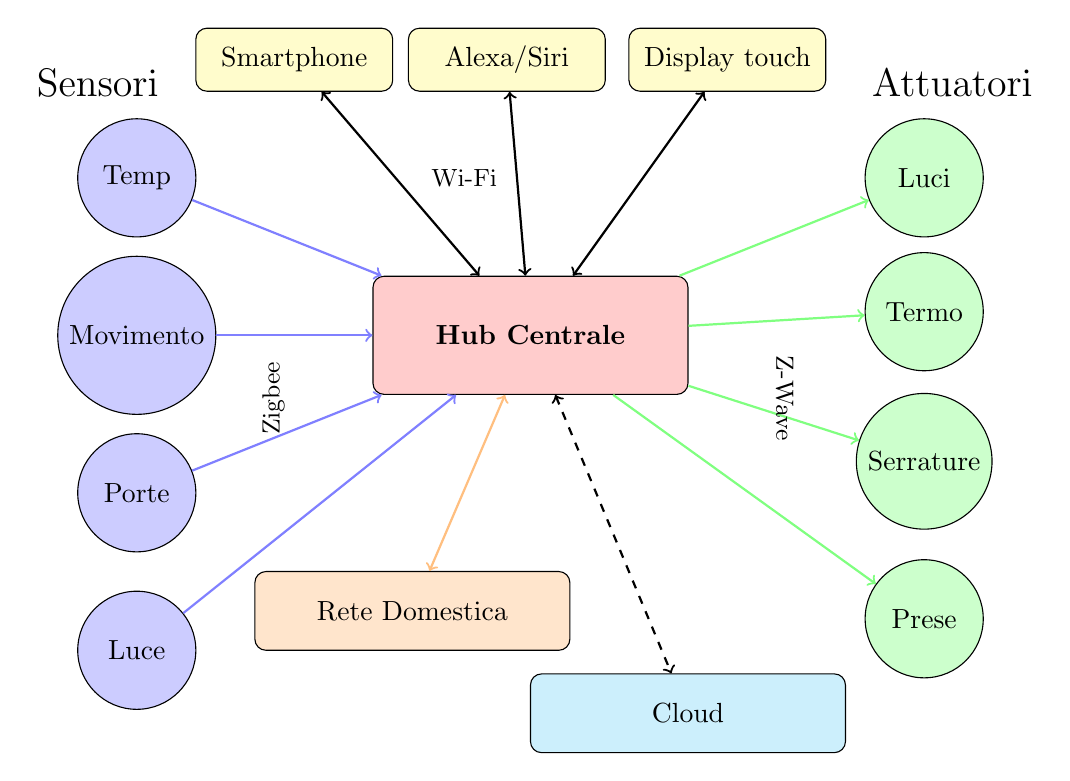
\begin{tikzpicture}[
    node distance=2cm,
    box/.style={rectangle, draw, rounded corners, minimum width=3cm, minimum height=1cm, text centered},
    sensor/.style={circle, draw, fill=blue!20, minimum size=1.5cm},
    actuator/.style={circle, draw, fill=green!20, minimum size=1.5cm},
    interface/.style={rectangle, draw, fill=yellow!20, rounded corners, minimum width=2.5cm, minimum height=0.8cm},
]

% Controller centrale
\node[box, fill=red!20, minimum width=4cm, minimum height=1.5cm] (hub) at (0,0) {\textbf{Hub Centrale}};

% Sensori (sinistra)
\node[sensor] (temp) at (-5,2) {Temp};
\node[sensor] (motion) at (-5,0) {Movimento};
\node[sensor] (door) at (-5,-2) {Porte};
\node[sensor] (light) at (-5,-4) {Luce};

% Attuatori (destra)
\node[actuator] (bulb) at (5,2) {Luci};
\node[actuator] (thermostat) at (5,0.3) {Termo};
\node[actuator] (lock) at (5,-1.6) {Serrature};
\node[actuator] (plug) at (5,-3.6) {Prese};

% Interfacce utente (sopra)
\node[interface] (app) at (-3,3.5) {Smartphone};
\node[interface] (voice) at (-0.3,3.5) {Alexa/Siri};
\node[interface] (wall) at (2.5,3.5) {Display touch};

% Cloud (sopra a destra)
\node[box, fill=cyan!20, minimum width=4cm] (cloud) at (2,-4.8) {Cloud};

% Rete locale (sotto)
\node[box, fill=orange!20, minimum width=4cm] (network) at (-1.5,-3.5) {Rete Domestica};

% Connessioni
% Sensori -> Hub
\foreach \s in {temp,motion,door,light}
    \draw[->, thick, blue!50] (\s) -- (hub);

% Hub -> Attuatori
\foreach \a in {bulb,thermostat,lock,plug}
    \draw[->, thick, green!50] (hub) -- (\a);

% Interfacce <-> Hub
\foreach \i in {app,voice,wall}
    \draw[<->, thick] (\i) -- (hub);

% Hub <-> Cloud
\draw[<->, thick, dashed] (hub) -- (cloud);

% Hub <-> Network
\draw[<->, thick, orange!50] (hub) -- (network);

% Etichette protocolli
\node[rotate=90, above] at (-3,-0.8) {\small Zigbee};
\node[rotate=-90, above] at (3,-0.8) {\small Z-Wave};
\node[left] at (-0.3,2) {\small Wi-Fi};
\node[left] at (-4.6,3.2) {\Large Sensori};
\node[left] at (6.5,3.2) {\Large Attuatori};

\end{tikzpicture}
\caption{Architettura tipica di un sistema domotico residenziale}
\label{fig:architettura-domotica}
\end{figure}

\subsection{Sensori}

I sensori servono a raccogliere le informazioni sull’ambiente circostante come ad esempio:

\begin{itemize}
    \item misuratorazione dell'ambiente (per la temperatura, l'umidità, la luminosità, la qualità dell’aria, etc.);
    \item rilevamento di movimento/presenza (PIR, microonde, ultrasuoni);
    \item controlli di sicurezza (controllano l'apertura porte/finestre, la presenza di fumo, gas, fuiriuscite di acqua);
    \item misuratorazione del consumo energetico.
\end{itemize}

\subsection{Attuatori}

Gli attuatori sono i dispositivi che trasferiscono i comandi ricevuti in azioni fisiche:

\begin{itemize}
    \item per accensione/spegnimento di luci e dispositivi;
    \item per il controllo di tapparelle, tende e infissi motorizzati;
    \item per la regolazione di riscaldamento e condizionamento;
    \item per la gestione di elettrodomestici e impianti multimediali.
\end{itemize}

\subsection{Controller e hub}

L’unità centrale (hub) è il vero e proprio cervello del sistema, deve gestire le regole di automazione, interpretare i dati e coordinare le azioni sugli attuatori. In alcuni casi può essere un dispositivo fisico dedicato, un assistente vocale (es. Alexa, Google Home) o un server locale (es. Home Assistant su Raspberry Pi).

\subsection{Interfacce utente}

Gli utenti possono interagire con il sistema tramite:

\begin{itemize}
    \item App mobili;
    \item Interfacce vocali;
    \item Dashboard web;
    \item Pulsanti intelligenti o pannelli touch.
\end{itemize}

\subsection{Reti di comunicazione}

La rete collega tutti i dispositivi tra di loro. Può essere cablata (es. KNX) o wireless (es. Zigbee, Z-Wave, Wi-Fi, Thread). I protocolli scelti influenzano la scalabilità, l’efficienza e la sicurezza del sistema.

\section{I vantaggi della domotica}

\subsection{Efficientamento energetico}

La domotica permette di gestire in maniera più consapevole i consumi energetici che vengono utilizzati dalla casa, tra questi possiamo avere:

\begin{itemize}
    \item la gestione e ottimizzazione del sistema di riscaldamento e del sistema di raffrescamento;
    \item il monitoraggio dei dispositivi inutilizzati e lo spegnimento automatico di luci;
    \item poter costruire una dashboard per monitorare i consumi in tempo reale.
\end{itemize}

\subsection{Sicurezza}

Grazie all'utilizzo dei sensori e alle automazioni è possibile ricevere notifiche rendendo la casa più sicura:

\begin{itemize}
    \item rilevamento intrusioni o incidenti (fumo, acqua, CO);
    \item gestione remota e controllo in tempo reale;
    \item registrazione video e notifiche intelligenti.
\end{itemize}

\subsection{Comfort e accessibilità}

L'automazione è alla base per la semplificazione la vita quotidiana:

\begin{itemize}
    \item scenari personalizzati (es. “buongiorno”, “cinema”);
    \item controllo vocale per utenti con disabilità;
    \item adattamento dinamico dell’ambiente alle esigenze familiari.
\end{itemize}

\section{Sfide attuali e prossimi capitoli}

Nonostante il progresso tecnologico ed alla riduzione dei costi, persistono però numerosi ostacoli ad un'adozione diffusa:

\begin{itemize}
    \item \textbf{Interoperabilità}: i dispositivi di marche diverse spesso non comunicano bene tra di loro
    \item \textbf{Sicurezza e privacy}: i dispositivi connessi devono proteggere i dati e gli accessi non autorizzati
    \item \textbf{Affidabilità}: un sistema domestico deve funzionare anche in caso di disconnessioni dalla rete o in caso di guasti di alcune sue componenti
\end{itemize}

Nel prossimo capitolo analizzeremo più da vicino le tecnologie di comunicazione che rendono possibile tutto questo, confrontando protocolli cablati e wireless in termini di prestazioni, consumo e compatibilità.

